\documentclass[letterpaper,12pt]{article}
\usepackage{tabularx} % extra features for tabular environment
\usepackage{amsmath}  % improve math presentation
\usepackage{float}
\usepackage{pdfpages}


\usepackage{graphicx} % takes care of graphic including machinery
\graphicspath{ {./figures/} }
%\usepackage[margin=1in,letterpaper]{geometry} % decreases margins
%\usepackage{cite} % takes care of citations
\usepackage[final]{hyperref} % adds hyper links inside the generated pdf file
\hypersetup{
	colorlinks=true,       % false: boxed links; true: colored links
	linkcolor=blue,        % color of internal links
	citecolor=blue,        % color of links to bibliography
	filecolor=magenta,     % color of file links
	urlcolor =blue         
}
\usepackage[margin = 1in,headsep=0.5cm,headheight=2cm,letterpaper]{geometry} 

\usepackage{fancyhdr}
\pagestyle{fancy}
\lhead{Student 1 : Ahmet Akman 2442366 \\ Student 2: Yusuf Toprak Yıldıran 2444149 }
\rhead{Date: \today \\ Group: Wednesday Morning - 5} 
%\cfoot{center of the footer!}
%\renewcommand{\headrulewidth}{0.1pt}



\begin{document}
\thispagestyle{empty}

\title{ \vspace{-2cm} Spring 2022 EE214 Project Work  \protect\\ Final Report\vspace{-4mm}}
\author{ Ahmet Akman 2442366 \protect\\ Yusuf Toprak Yıldıran 2444149 }
\date{}
\maketitle
%\tableofcontents
%\begin{abstract}
%abstract
%\end{abstract}
\section{Introduction}

In this document we present our work done to satisfy the requirements of the Term Project of EE214 laboratory course. According to the project description we are supposed to make a transmitter which produces different frequency tones (pure sinusoids) and collect them together, and a receiver which can be tuned to these frequencies. The received tone will be played with a speaker.
So, in order to overcome the challange of generating sinusoids with needed frequencies the square wave generator circuits are used. In the receiver unit , the bandpass filter with topology called dual-opamp is used as planned in the Preliminary Report. For the speaker unit a simple opamp amplifier is utilized. 


\section{Transmitter Unit}
In the transmitter unit, sinusoidal signals with frequencies 1\(kHz\), 2\(kHz\), 3\(kHz\), 5\(kHz\), 6\(kHz\), 7\(kHz\), 9\(kHz\), 10\(kHz\), 11\(kHz\), 13\(kHz\), 14\(kHz\), 15\(kHz\) are aimed to be produced and then collected into a single waveform by avoiding to produce 4\(kHz\), 8\(kHz\), 12\(kHz\) frequencies. 

\subsection{Astable Multivibrator}
In order to obtain a waveform that includes these all 12 sinusoids with different frequencies, 1\(kHz\) and 2\(kHz\) square waves are considered to be summed up based on the idea fourier transformation. The reason behind this is that the summing of sinusoids with frequencies 1\(kHz\), 3\(kHz\), 5\(kHz\), 7\(kHz\), 9\(kHz\), 11\(kHz\), 13\(kHz\), 15\(kHz\) results in 1\(kHz\) square wave waveform and similarly summing of the rest of the sinusoidal signals that must be produced is result in a 2\(kHz\) square wave signal. For this to be achieved, 2 square wave generator circuits were designed to generate 1\(kHz\) which is given in Figure 1, and 2\(kHz\) given in Figure 2 square waves. Since higher frequencies that constitute the square wave are low in their magnitude, generating and filtering them precisely is harder. Therefore, for example, one needs to generate 1\(kHz\) square wave precisely to be able to include a nice 13\(kHz\) and 15\(kHz\) sine waves.
Also in order to be able to generate a square wave with smaller rise and fall time tl071 op-amp (\href{https://www.st.com/resource/en/datasheet/tl071.pdf}{datasheet} ) which has a big slew rate is used. Additionally for the same reason BS-170 (\href{https://www.onsemi.com/pdf/datasheet/mmbf170-d.pdf}{datasheet} )N channel enhancement mode MOSFETs are used as an inverter.  

Frequency of the generated signal is calculated as follows when the necessary analysis is made:
\begin{center}
    $ \frac{1}{2RC} $
\end{center}
where R is equivalent resistance between output and non-inverting terminals of the op-amp.
\begin{figure}[H]
    \centering
    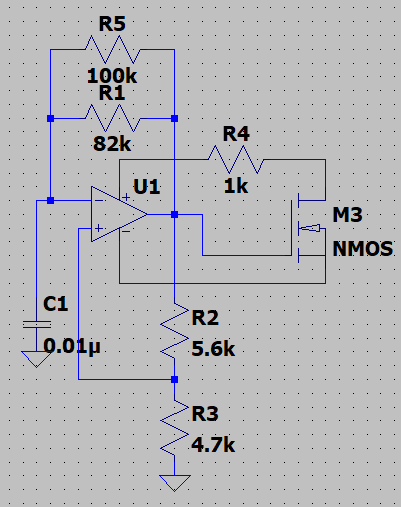
\includegraphics[width = 0.75\textwidth]{1K.png}
    \caption{Op-amp Multivibrator for 1\(kHz\)}
\end{figure} 



\begin{figure}[H]
    \centering
    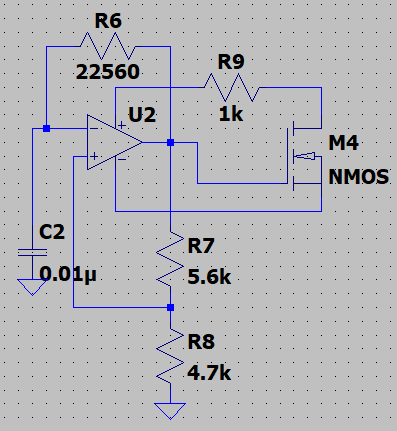
\includegraphics[width = 0.75\textwidth]{2K.png}
    \caption{Op-amp Multivibrator for 2\(kHz\)}
\end{figure} 


\subsection{Summing Amplifier}
After generating two square waves with the necessary sines, there needs to be a summing amplifier to obtain one single waveform. This is made by setting a summing op-amp circuit given in Figure 3 which gives an output equals to \(- \frac{10k\Omega }{2.2k\Omega }(V_1 + V_2)\) where \(V_1\) and \(V_2\) are the outputs of the signals with  1\(kHz\) and 2\(kHz\) frequencies respectively.


\begin{figure}[H]
    \centering
    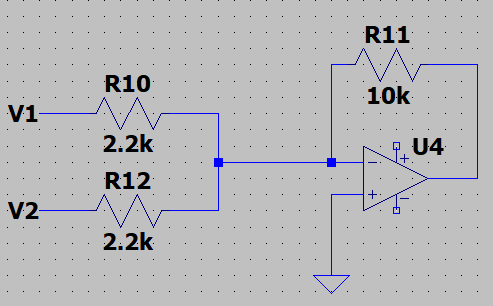
\includegraphics[width = 0.75\textwidth]{SUMM.png}
    \caption{Summing Amplifier Circuit}
\end{figure} 

\section{Receiver Unit}
In the receiver unit design phase, the design path described in the Preliminary report is followed. The reference point for the filter design was primarily the \href{https://www.analog.com/media/en/training-seminars/design-handbooks/basic-linear-design/chapter8.pdf}{analog filter design guide} prepared by Analog Devices company.
\subsection{Dual-Opamp Topology}
The reason why the dual-opamp bandpass filter is used is there are only two resistors that adjust the frequency, and fixing the value of the one is acceptable. Also, the quality factor can be adjusted almost independently from the resonant frequency. The transfer function of this topology can be expressed as follows;
\begin{center}
    $ \frac{H \omega_0^2 }{s^2 + \alpha \omega_0 s + \omega_0 ^2} $
    
\end{center}
The general schematic of the topology is given in Figure X .
\begin{figure}[H]
    \centering
    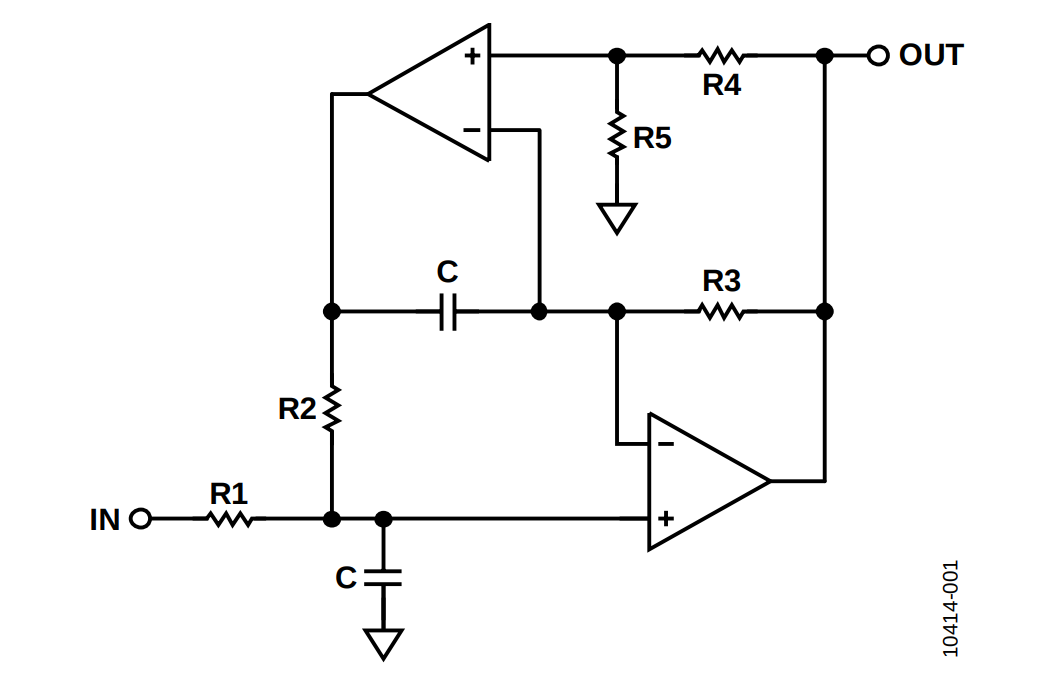
\includegraphics[width = 0.75\textwidth]{dualopamp.png}
    \caption{Dual-opamp topology schematic}
\end{figure} 
\subsection{Compononent Selection and Simulation Results}
To be able to adapt the circuit efficiently to our purpose following goals are set. The design tables for the standard responses are not used to choose the component values freely. Instead, the responses are obtained through multiple simulations.
\begin{itemize}
    \item The values of the passive components should be easy to supply.
    \item The R3 should be fixed so that the highest Q is obtained for 14-15 kHz frequencies since the harmonics of the transmitter signal are quite small compared to the 1 and 2 kHz.
\end{itemize}
So the values of R4 and R5 are fixed to 1k, and R1 is fixed to 100K. The capacitors are fixed to 10nF. Then series of simulations are made to find a suitable value for R3, which is fixed to 1K for better amplification of 14-15 kHz signals. Lastly, the values of the R2 are fine-tuned for every frequency. This is also important to determine which range of potentiometers to be used. The circuit schematic of the receiver is given in Figure X.
\begin{figure}[H]
    \centering
    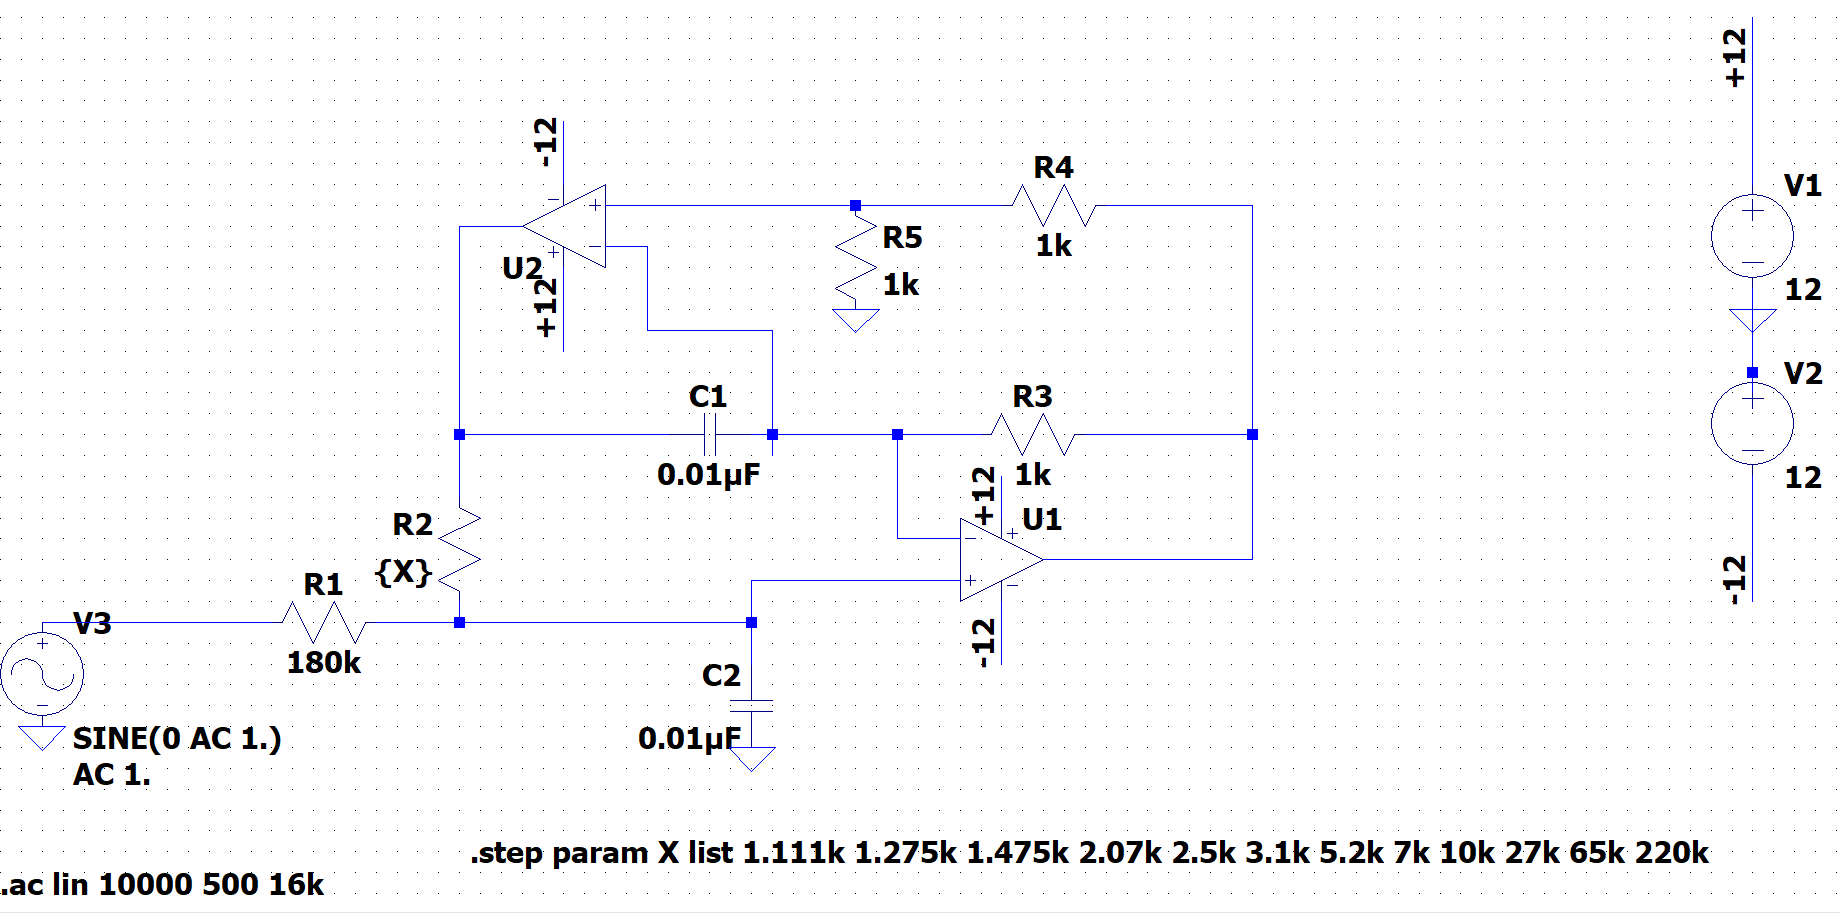
\includegraphics[width = 0.75\textwidth]{receiver_schematic.png}
    \caption{Receiver circuit schematic.}
\end{figure}

The frequency response for the receiver circuit obtained in LTSpice is given in Figure X.
\begin{figure}[H]
    \centering
    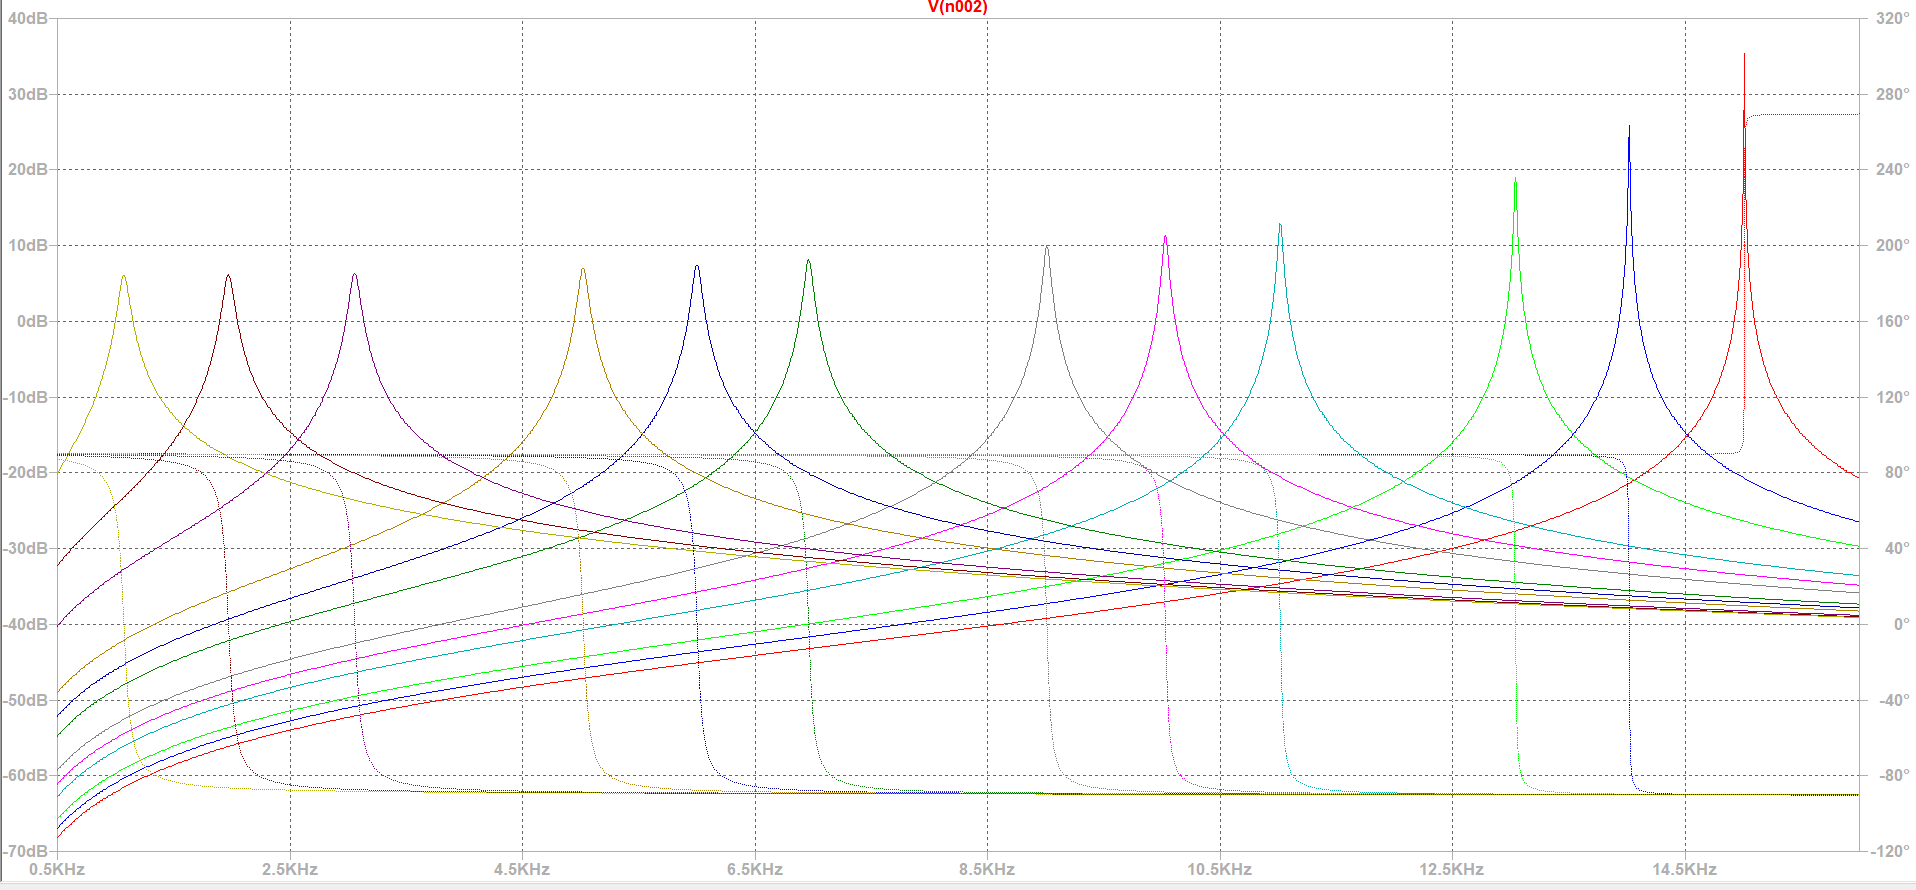
\includegraphics[width = 0.75\textwidth]{response.png}
    \caption{Receiver circuit frequency response.}
\end{figure}
\section{Physical Prototype and Results}
To be able to construct the designed circuit LM358 (\href{https://pdf.direnc.net/upload/lm358-datasheet.pdf}{datasheet}two opamp packaged in an ic ) are used. To ensure an average of two opamp ic is sufficient to accomplish the needed filtering, double opamp ic's with the same pinout TL072 and TL082 are tested and obtained the same result. The physically prototyped version of the circuit is given in Figure X.
\begin{figure}[H]
    \centering
    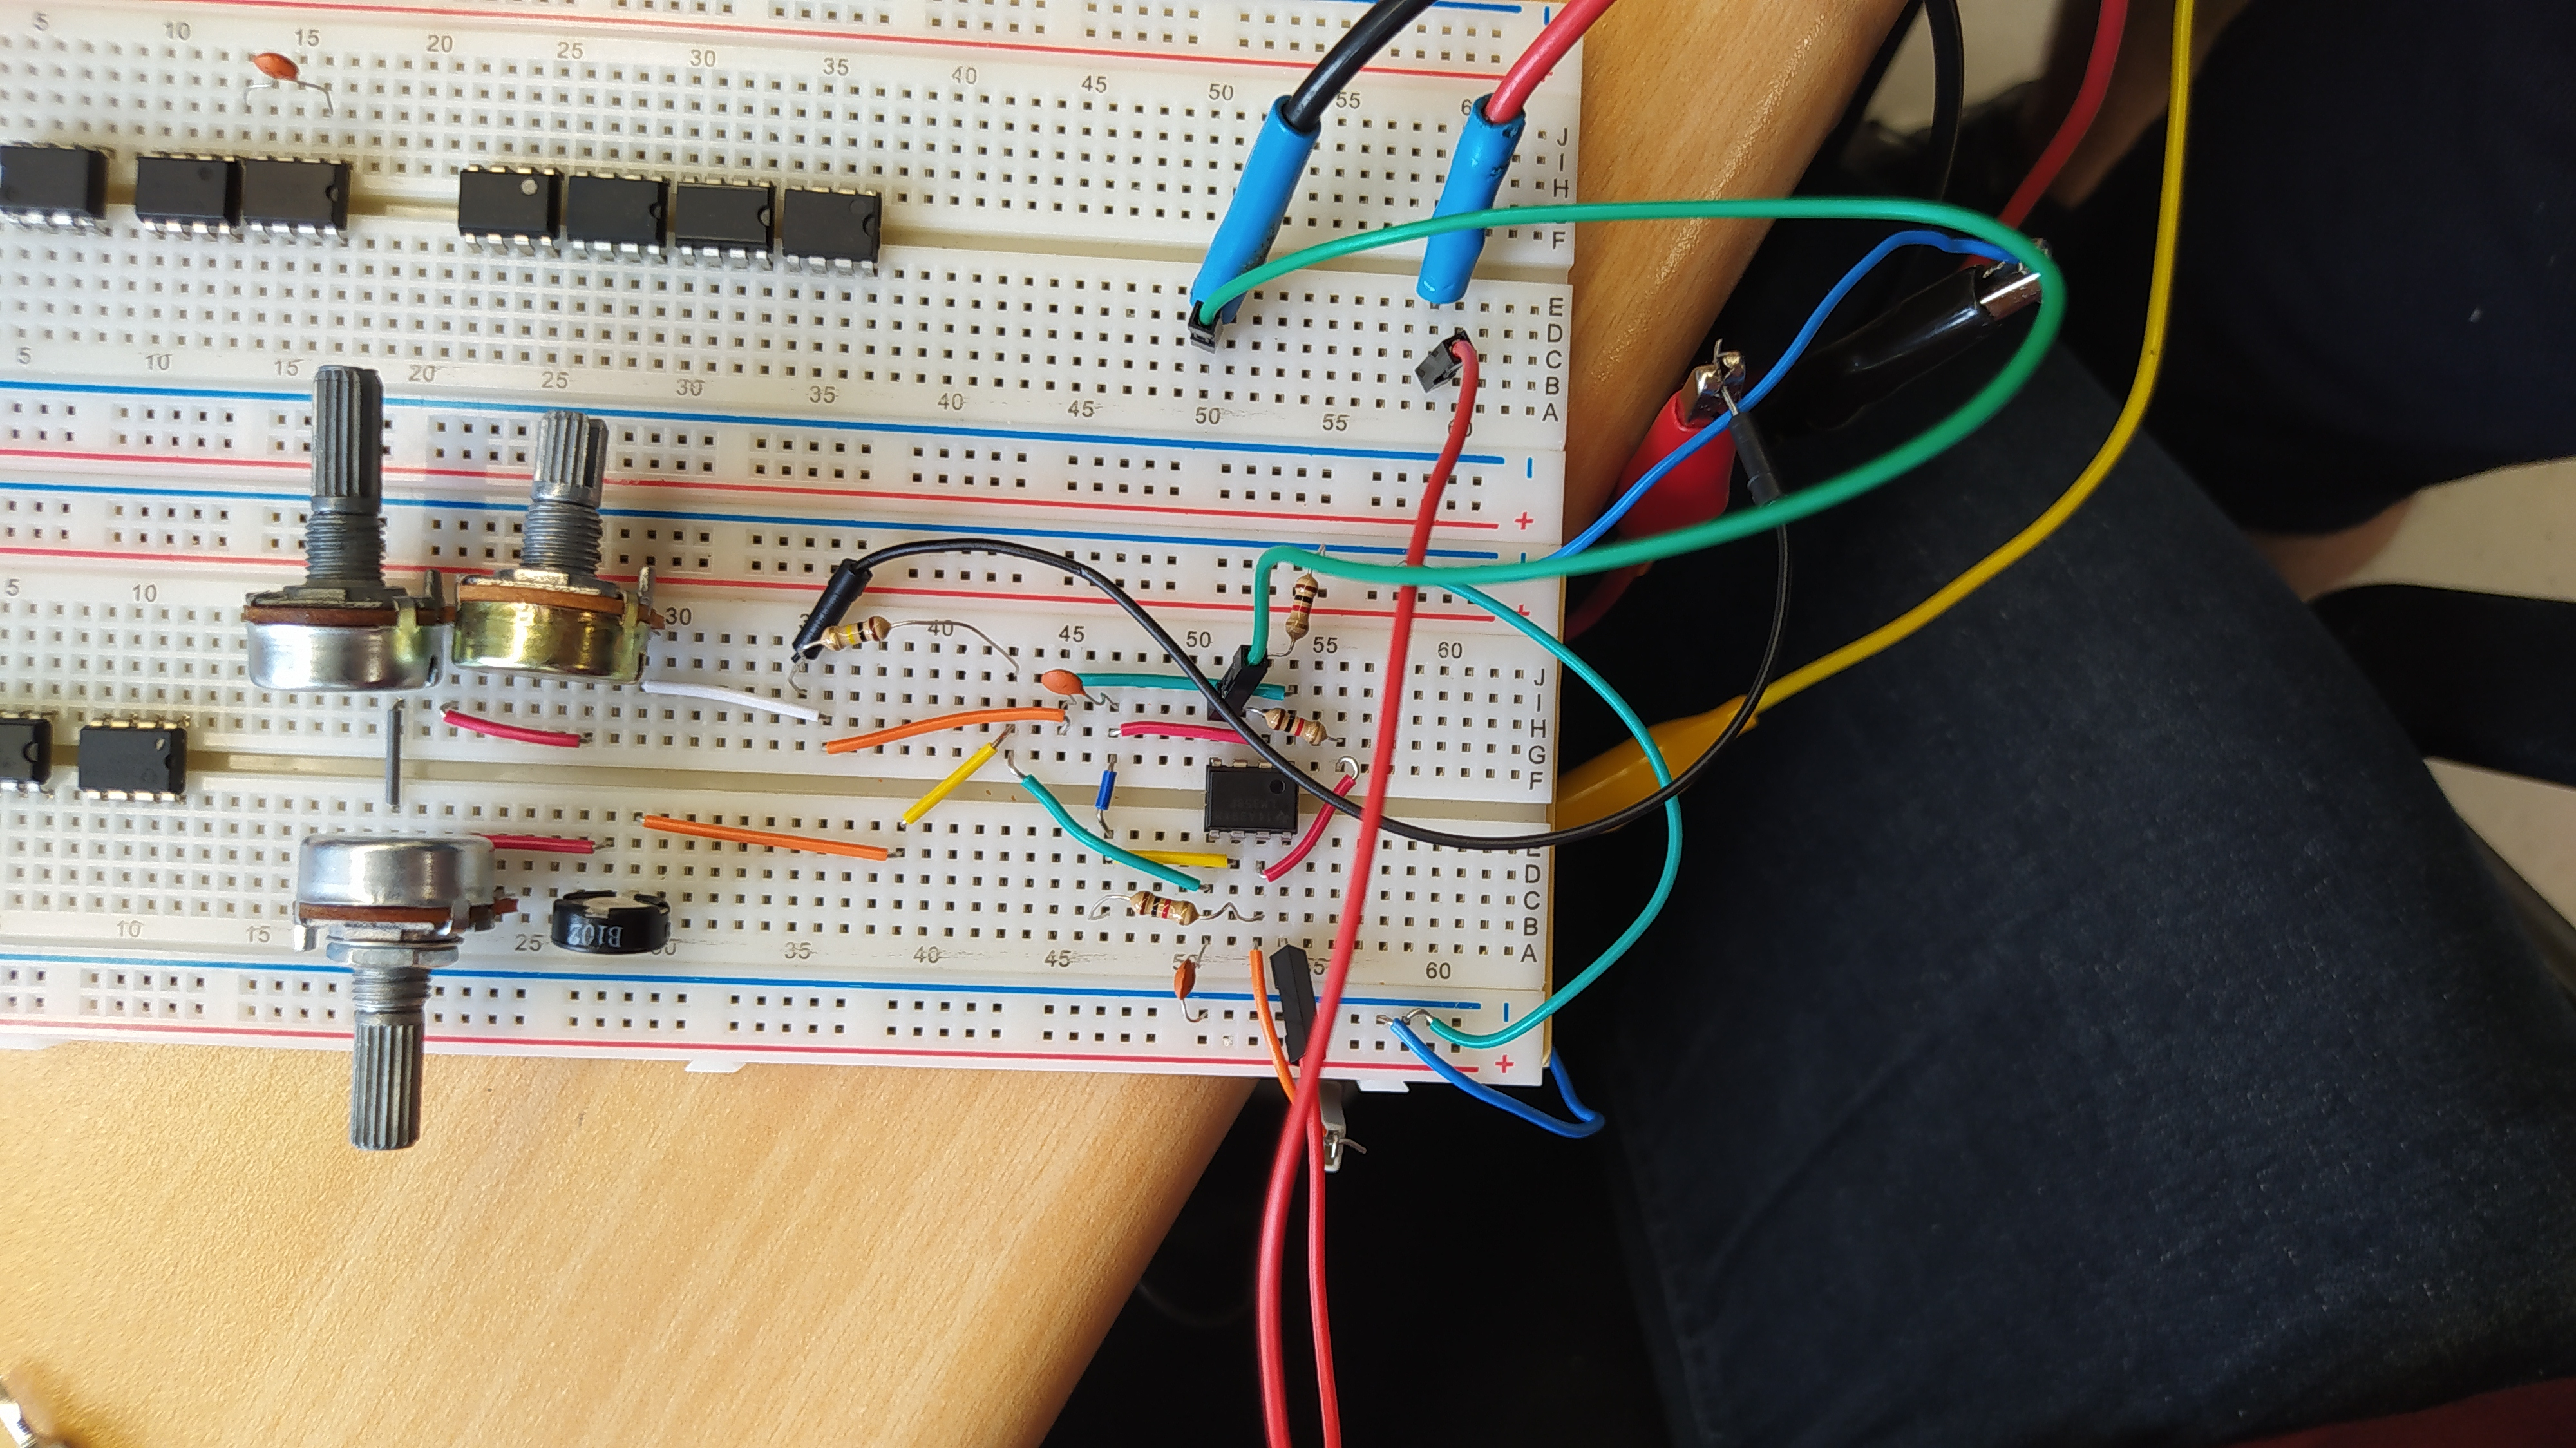
\includegraphics[width = 0.75\textwidth]{receiver_bread.jpg}
    \caption{Receiver Unit Breadboard}
\end{figure}
Four potentiometers with 1K, 10K, 50K, and 250K are used in series for R2 to fine-tune the middle frequencies. So the one potentiometer bonus is achieved.
As a result, an analog bandpass filter with adjustable middle frequency is obtained successfully. The filter is able to filter all needed signals accurately with approximately 30-40 dB difference. The output amplitude of the filter ranges from 6 Vpp to 2Vpp. 
\section{Speaker Unit}
For the speaker unit, a simple approach is followed. Since the transmitter has decreasing harmonics amplitude and the receiver has increasing gain for increasing frequencies, the speaker amplification need not be higher than 2X. Also, a headphone speaker with 32R impedance is used, which has not needed for high current flow. As a result, an inverting opamp amplifier is used. The schematic is given in Figure X.
\begin{figure}[H]
    \centering
    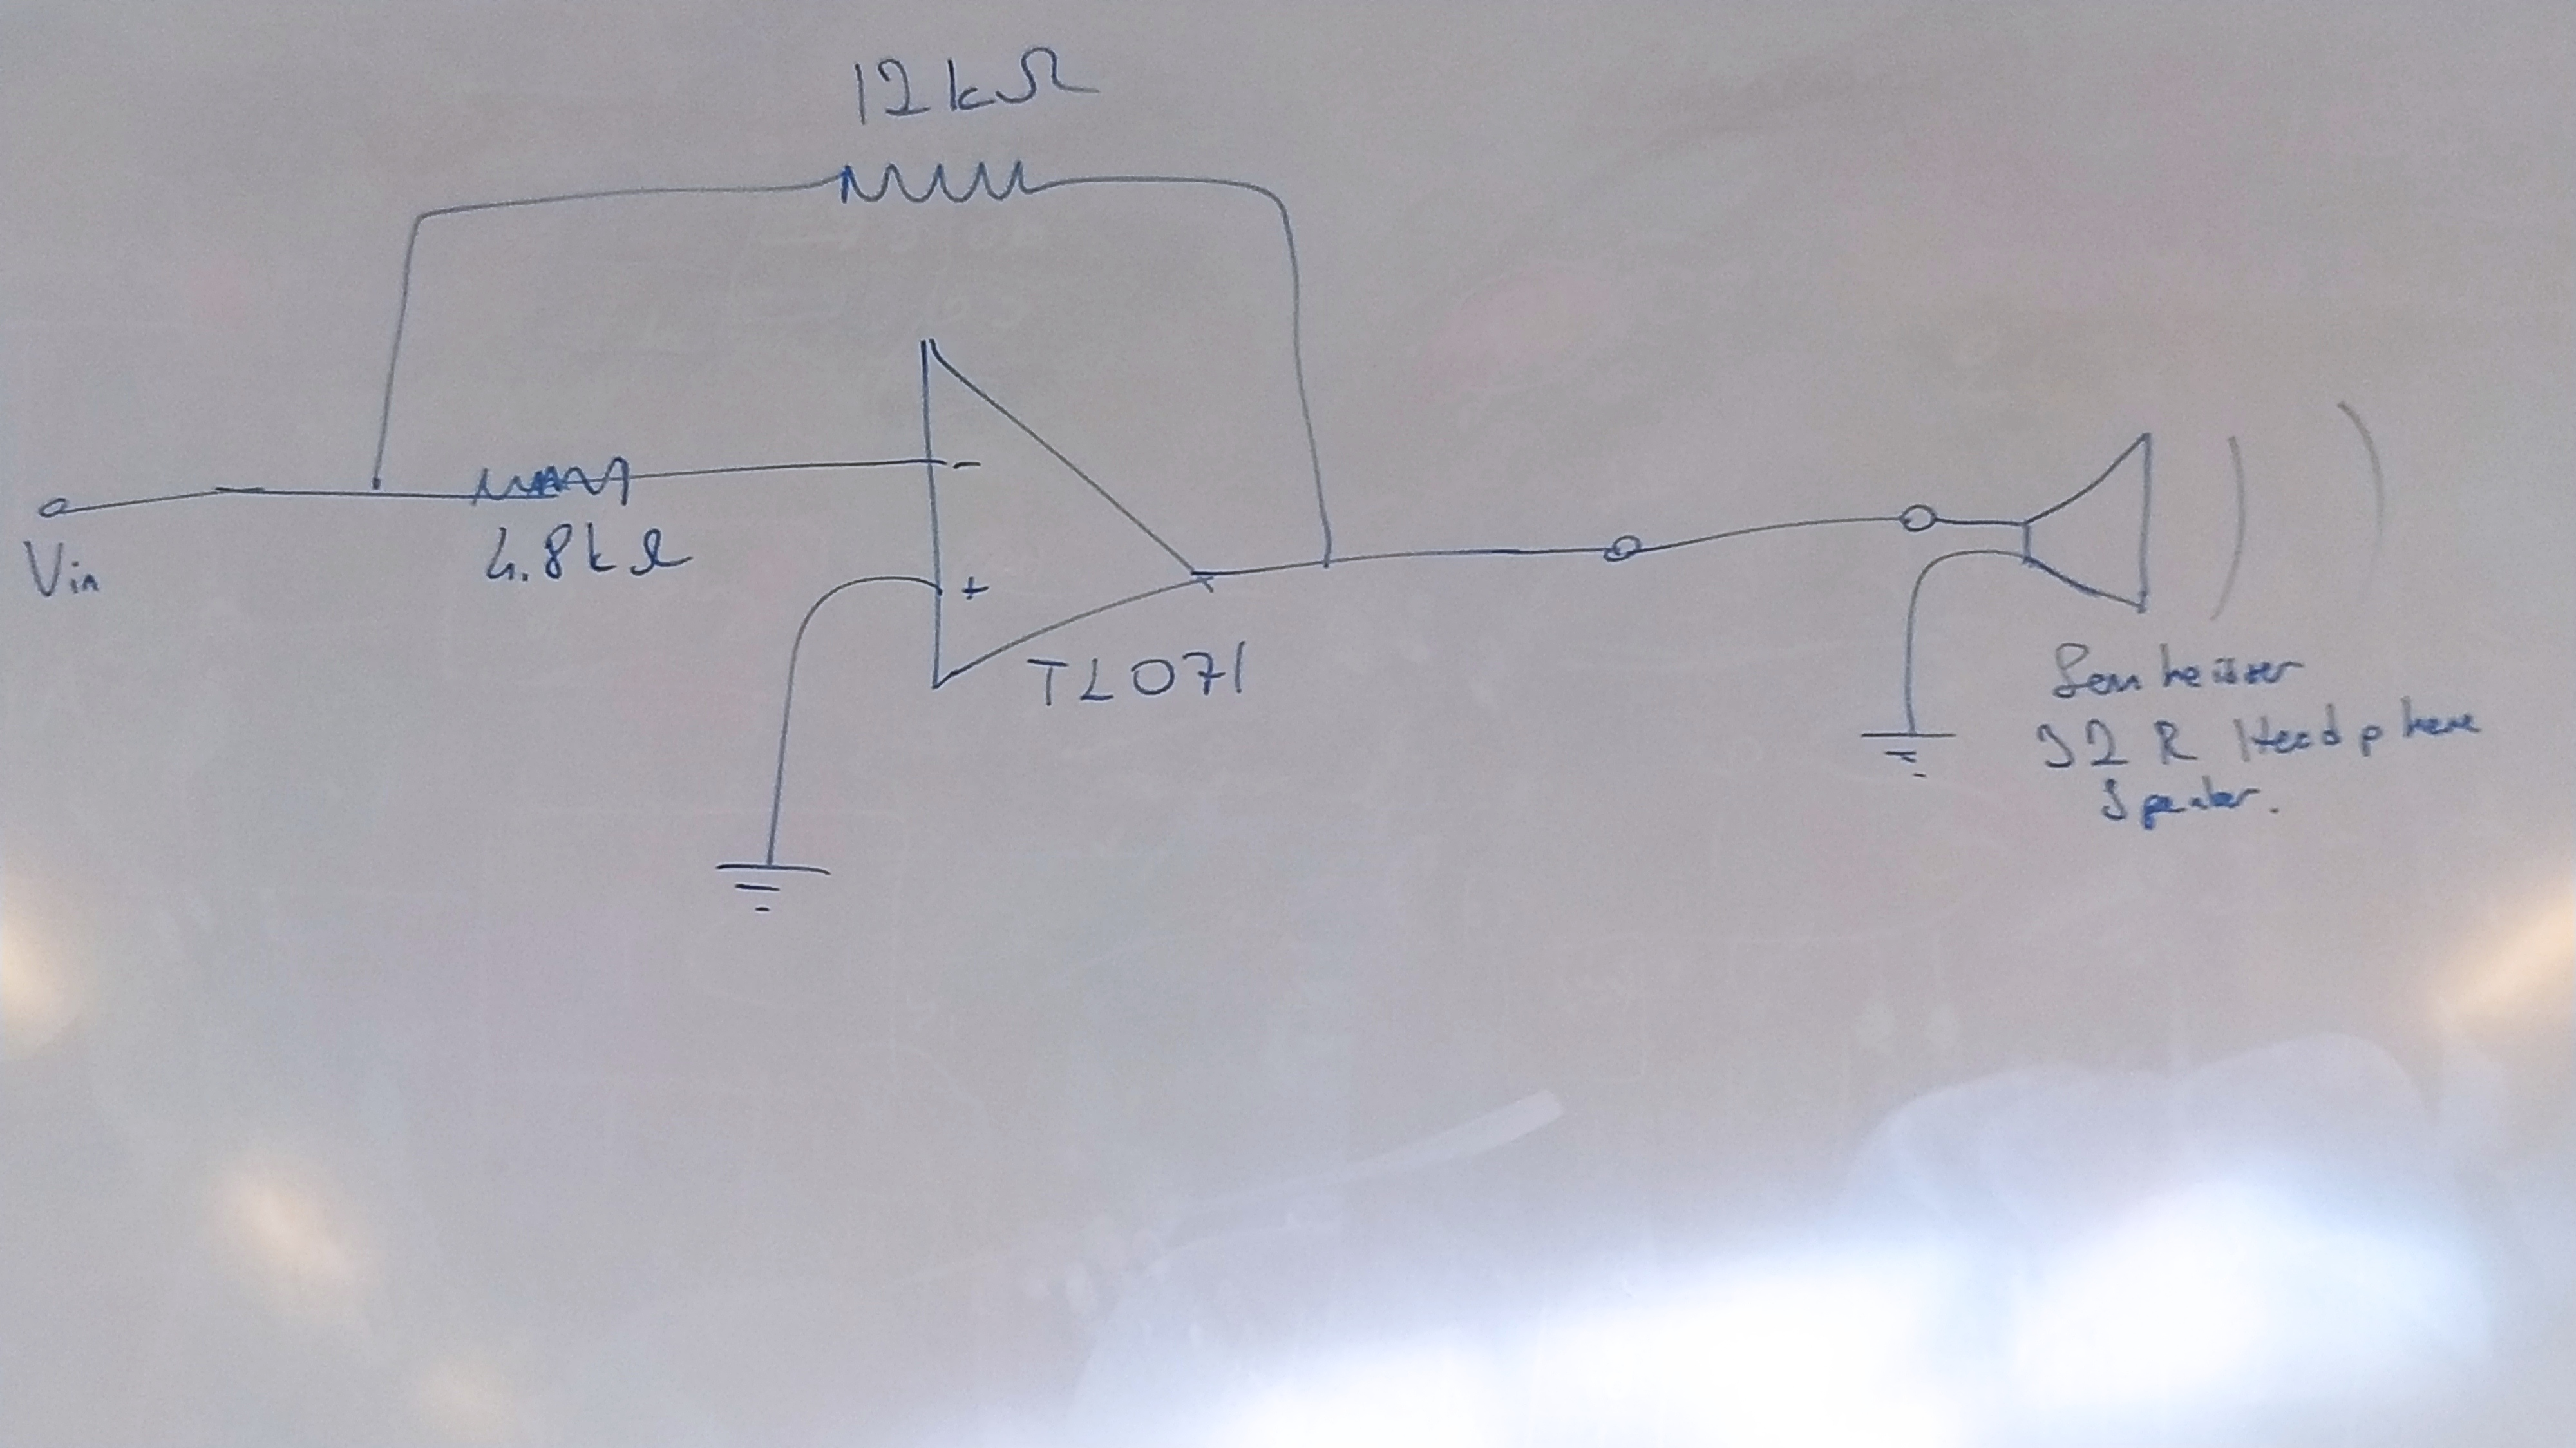
\includegraphics[width = 0.75\textwidth]{speaker_schematic.jpg}
    \caption{Speaker unit schematic}
\end{figure}

As a result, all needed signals are quite audible with (almost) sine tonality. 

\section{Conclusion}
To conclude, EE214 Term Project is presented in this document by explaining generating, collecting, and filtering process of sinusoidal signals with 12 different frequencies. In order to obtain well results more appropriate components are preferred and additive circuit designs (such as MOSFET inverter) are used in order to obtain nice signals. Afterward, a filter circuit with dual-opamp topology is set. Lastly, a speaker unit is set using an amplifier circuit since there needs a matching between impedances of speaker input and the rest of the circuit.    

\end{document}

%%%%%%%%%%%%%%%%%%%%%%   EXAMPLE TABLE   %%%%%%%%%%%%%%%%%%%%%%%%%%%%%%%%
\begin{table}[H]
\begin{center}
    \caption{Resistance reading by color code convention.}
    \vspace{2mm}
    \begin{tabular}{||c | c | c||} 
        \hline
        Color Order & Value & Tolerance \\ [0.5ex] 
        \hline\hline
        Brown / Black / Red / Gold & 1k\( \Omega \) & \( \% \) 5  \\ 
        \hline
        Yellow / Violet / Red / Gold & 4.7k\( \Omega \) & \( \% \) 5   \\
        \hline
        Brown / Grey / Orange / Gold & 18k\( \Omega \) & \( \% \) 5  \\ [1ex] 
        \hline
    \end{tabular}
\end{center}
\end{table}


%%%%%%%%%%%%%%%%%%%%%%   EXAMPLE IMAGE   %%%%%%%%%%%%%%%%%%%%%%%%%%%%%%%%
\begin{figure}[H]
\centering
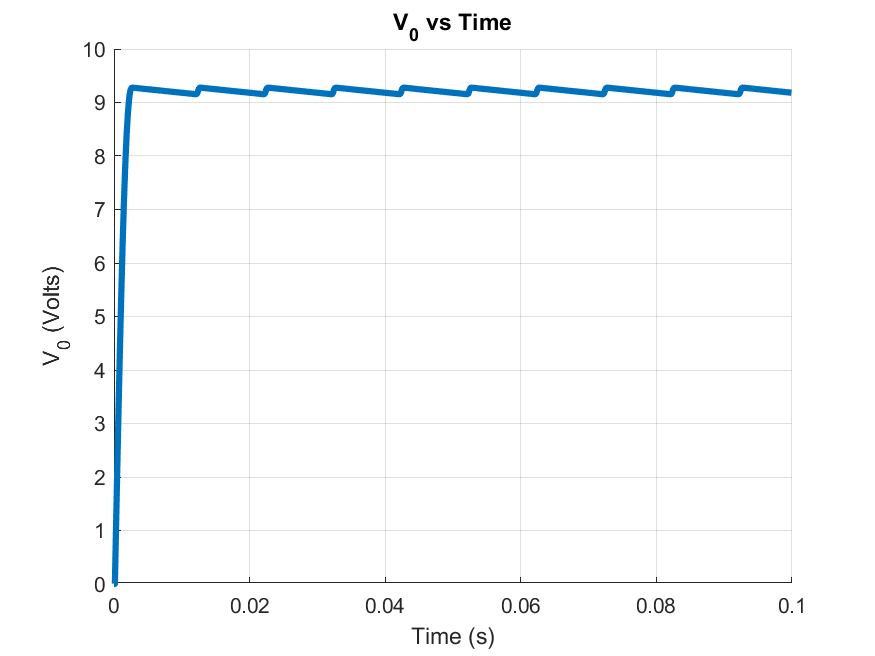
\includegraphics[width = 0.75\textwidth]{5.png}
\caption{Circuit schematic for the step 5}
\end{figure} 

%%%%%%%%%%%%%%%%%%%%%%   EXAMPLE IMAGE FROM PDF   %%%%%%%%%%%%%%%%%%%%%%%%%%%%%%%%
\begin{figure}[H] \centering{
	\includegraphics[scale=0.25]{2a_plot.pdf}}
	\caption{Experiment 2}
\end{figure}
%%%%%%%%%%%%%%%% Deneme Push